\subsection{Bahnplanung}
Zunächst einige relevante Definitionen:
\begin{itemize}
\item \red{Konfiguration $K$}: vollständige, eindeutige Beschreibung
des Zustands eines Roboters $A$, z.B.
\begin{itemize}
\item im euklidischen Raum durch seine Position und Orientierung
\item im Gelenkwinkelzustandsraum durch die Werte der Gelenke
\end{itemize}
\item \red{Konfigurationsraum $IK$}: Raum aller
möglichen Konfigurationen des Roboters $A$
\item \red{Weg} des Roboter $A$ von der Konfiguration $K_{Start}$ zu $K_{Ziel}$ ist eine stetige Abbildung:
\begin{align*}
\tau: [0, 1] \rightarrow \mathbb{K}\\
\tau(0) = K_{Start} ,\tau(1) = K_{Ziel}
\end{align*}
\item \red{Einschränkung} für den Roboter $A$ ist eine Abbildung:
\begin{align*}
\lambda : \mathbb{K} \rightarrow [0, 1]
\end{align*} 
\item \red{Arbeitsraumhindernis $H$}: Raum, welcher von
einem Objekt im Arbeitsraum eingenommen wird
\item \red{Konfigurationsraumhindernis $\mathbb{K}_{H_i}$}: Menge aller
Punkte des Konfigurationraumes, welche innerhalb eines
Arbeitsraumhindernisses $H_i$ liegen:
\begin{align*}
\mathbb{K}_{H_i} = {K \in \mathbb{K} | K \in H_i}
\end{align*}
\item \red{Hindernisraum $\mathbb{K}_{H_i}$}: Menge aller
Konfigurationsraumhindernisse:
\begin{align*}
\mathbb{K}_H =\bigcup_i \mathbb{K}_{H_i}
\end{align*}
\item \red{Freiraum $\mathbb{K}_F$}: Menge aller Punkte aus $\mathbb{K}$, welche nicht im
Hindernisraum liegen:
\begin{align*}
\mathbb{K}_F = \mathbb{K}\backslash \mathbb{K}_H
\end{align*}
\item \red{kollisionsfreier Weg $\tau$}: Weg mit $Bild(\tau) \subseteq \mathbb{K}_F$, also ein Pfad welcher alle Einschränkungen erfüllt
\end{itemize}
Bei einer Bahnplanung im Konfigurationsraum werden Bewegungen eines Roboters als \red{Trajektorie im Konfigurationsraum}, d.h. als Zustandsänderungen über die Zeit
relativ zu einem stationären Koordinatensystem (kartesischer Raum, Gelenkwinkelraum) aufgefasst:
\begin{itemize}
\item Gegeben: $K_{Start}$ = Startkonfiguration, $\land_{Ziel}$ = Menge der Zieleinschränkungen
\item Gesucht: Kollisionsfreier Weg $\tau$ von $K_{Start}$ nach $K$ mit $\lambda(K)=1 \forall \lambda \in \land_{Ziel}$
\item Bedingungen: i.A. Gütekriterien, Neben-,Rand- sowie Zwangsbedingungen
\end{itemize}
Hierbei sei angemerkt, dass von Roboter und Umwelt zu einem Punkt im Konfigurationsraum abstrahiert wird. Die Kollisions- bzw. Einschränkungsüberprüfung stellt eine Blackbox
\begin{align*}
f: \mathbb{K} \rightarrow \{0, 1\}\\
\text{Beispiel:} f(K) = \bigwedge\limits_{\varv \in \land_{Weg}}^{} \varv(K) \geq \varepsilon(\varv)
\end{align*}
dar. Bei Entwicklung allgemeiner Planungsverfahren auf Basis dieser Abstraktion entspricht die Bahnplanung einer Suche nach einer stetigen Verbindung zweier Punkte im
Konfigurationsraum. Eine explizite Beschreibung des Freiraums ist nicht notwendig, d.h. das Suchverfahren ist unabhängig von der Struktur und Repräsentation des Freiraums.

\subsubsection*{Simpler Rapidly-exploring Random Tree (RRT) Planer}
\paragraph*{RRT-Algorithmua}
Wie bereits zu Anfang des Kapitels erwähnt bringt die humanoide Servicerobotik zahlreiche Anforderungen mit sich, sowie die Manipulation beliebiger Objekte, das selbstständige Lösen komplexer Aufgaben und denj Einsatz im menschlichen Umfeld, d.h. humanoide Serviceroboter müssen in einer sehr komplexen Umgebung agieren und verfügen über sehr viele Freiheitsgrade (der Roboter Albert II beispielsweise hat 13df,  6 im Arm, 3 in der Plattform und 4 in der Hand. Daraus ergibt sich ein 13-dimensionaler Konfigurationsraum $\mathbb{R}^{13}$ als reellwertige Grundlage).
Ein Bahnplanungsalgorithmus, der hiermit umgehen kann ist der RRT = Rapidly-exploring Random Tree\footnote{[LaValle/Kuffner99]: Randomized Kinodynamic
Planning}, welcher zur effizienten Durchsuchung hoch-dimensionaler Räume entwickelt wurde. Er ist geeignet für holonome und nicht-holonome Problemstellungen mit Einschränkungen. Es wird inkrementell eine Baumstruktur aufgebaut und dabei der erwartete Abstand eines Punkts zu einem Knoten im Baum minimiert. Wenn die Zeit $t$ gegen unendlich geht kommt man beliebig nah an jeden beliebigen Punkt. Der Algorithmus erreicht eine hohe Geschwindigkeit durch schnelles Wachstum in nicht explorierte Bereiche. Die Wurzel ist ein Punkt im 13-dimensionalen Konfigurationsraum. Pseudocode ist in Algorithmus \ref{alg:rrt}. 
Eine graphische Veranschaulichung zeigt Tabelle \ref{tab:rrt}.
Der Knoten mit der größten Voronoi-Region hat jeweils die größte Wahrscheinlichkeit, als nächstes erweitert zu werden (Voronoi-Bias). Da am Anfang die Voronoi-Gebiete am
Randbereich groß sind findet zunächst eine rasche Exploration und dann eine Verfeinerung statt.
\begin{algorithm}
  \caption{RRT
    \label{alg:rrt}}
  \begin{algorithmic}[1]
    %\Require{$x$ and $y$ are packed \DNA strings of equal length $n$}
    %\Statex
    \Statex {BUILD\_RRT}($K_{Start}, n, \varepsilon$)
      \State T.init($K_{Start}$) \Comment{Neuer Baum mit Startkonfiguration in der Wurzel}
      \For{$k = 1 \textrm{ to } n$}
        \Let{$K_{Zuf}$}{RAND\_CONF()} \Comment{Gleichverteilt zufällige Erzeugung einer Konfiguration}
        \Let{$K_{Nahe}$}{NEAREST\_VERTEX($K_{Zuf}, T$)} \Comment{Bestimmung des nächsten Knotens}
        \Let{$K_{Neu}$}{EXTEND($K_{Nahe}, K_{Zuf}, \varepsilon$)} \Comment{Erzeugung einer neuen Konfiguration}
        \State T.add\_vertex($K_{Neu}$)
        \State T.add\_edge($K_{Nahe}, K_{Neu}$)
      \EndFor
      \State \Return{T}
    %\EndFunction
  \end{algorithmic}
\end{algorithm}

%Beispiel für Verwendung des Algorithmus-Packages
%\begin{algorithm}
%  \caption{Counting mismatches between two packed \DNA strings
%    \label{alg:packed-dna-hamming}}
%  \begin{algorithmic}[1]
%    \Require{$x$ and $y$ are packed \DNA strings of equal length $n$}
%    \Statex
%    \Function{Distance}{$x, y$}
%      \Let{$z$}{$x \oplus y$} \Comment{$\oplus$: bitwise exclusive-or}
%      \Let{$\delta$}{$0$}
%      \For{$i \gets 1 \textrm{ to } n$}
%        \If{$z_i \neq 0$}
%          \Let{$\delta$}{$\delta + 1$}
%        \EndIf
%      \EndFor
%      \State \Return{$\delta$}
%    \EndFunction
%  \end{algorithmic}
%\end{algorithm}
\begin{center}
\begin{table}[hbt]
\begin{tabular}{p{10cm}}
\centering
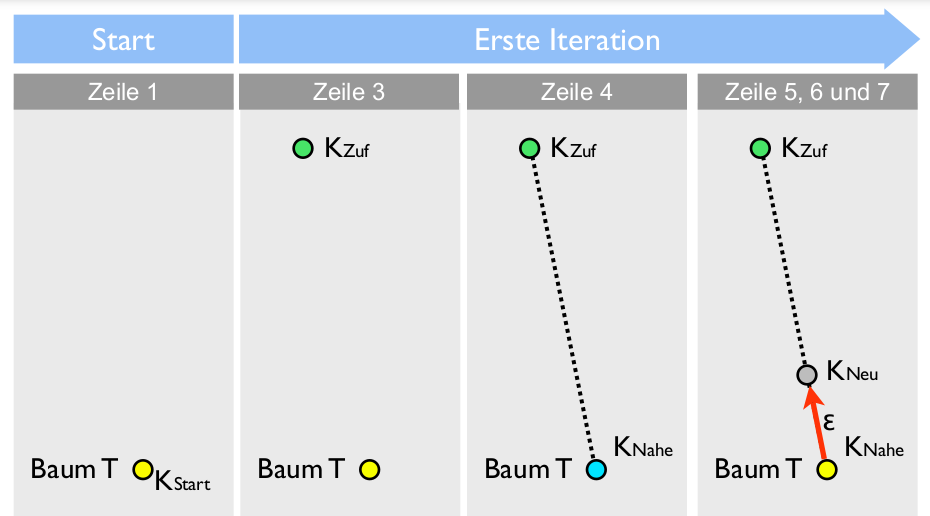
\includegraphics[width=1.5\linewidth]{figures/ch04_rrt1.png}\\
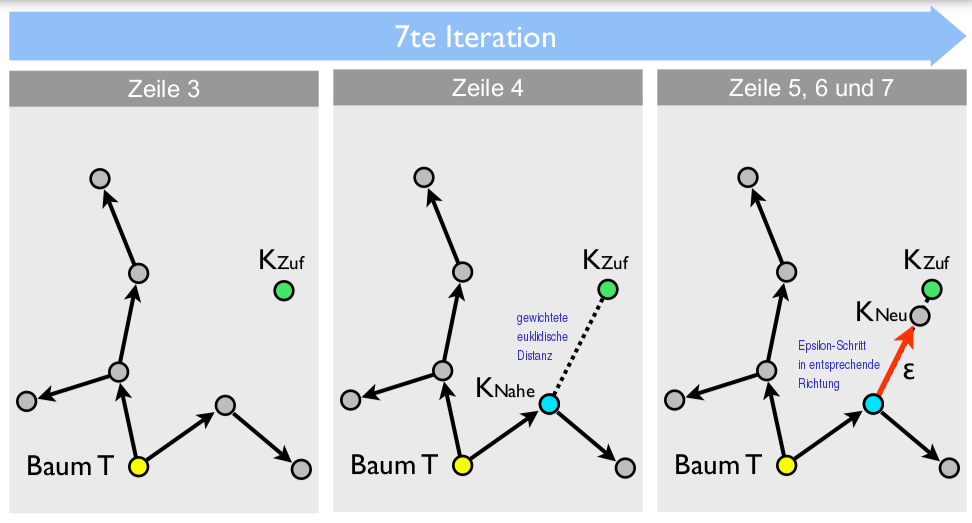
\includegraphics[width=1.5\linewidth]{figures/ch04_rrt2.png}
\end{tabular}
\caption{Graphische Veranschaulichung - RRT}
\label{tab:rrt}
\end{table}
\end{center}

RRT: Zusammenfassung
\begin{itemize}
\item Allgemeines Verfahren zur Durchsuchung hoch-dim. Räume
\item Online-Verfahren
\item Approximation des Suchraums durch eindimensionale Struktur: Baum
\item Rasche Exploration des Suchraums: Voronoi-Bias
\item Probabilistische (oder deterministische) Stichprobenerzeugung
\item Einfach zu implementieren, nur wenige Parameter ($\varepsilon$, Distanzfunktion auf $\mathbb{K}$)
\end{itemize}
\paragraph{Anwendung in der Bahnplanung} Es sind drei Fragen zu klären:
\begin{itemize}
\item Wie zielgerichtet suchen?
\item Wie kollisionsfreie Wege erzeugen?
\item Wie Einschränkungen berücksichtigen?
\end{itemize}
Hierzu muss der Basisalgorithmus erweitert werden:
\begin{itemize}
\item Es werden nur Konfigurationen hinzugefügt, die alle Einschränkungen erfüllen.
\begin{itemize}
\ita $K_{Neu}$ wird übernommen, wenn alle Einschränkungen zwischen $K_{Nahe}$ nach $K_{Neu}$ erfüllt sind
\ita Keine Distanz, nur Ja / Nein
\ita Kollisionen auf Grundlage eines Geometriemodells der Objekte (Standard: 3D-Dreiecksnetze)
\ita Kollisionsüberprüfung: mindestens zwei Dreiecke schneiden sich (oder 1. Objekt in 2. komplett enthalten), hierzu gibt es optimierte Algorithmen, ist vergleichsweise langsam
\end{itemize}
\item Bei der Stichprobenerzeugung werden mit einer bestimmten Wahrscheinlichkeit Zielkonfigurationen generiert, der Baum wächst in die Richtung der Zielkonfigurationen.
\item Der Planungsprozess ist beendet, wenn die letzte Konfiguration die Zieleinschränkungen erfüllt.
\end{itemize} 
\subsubsection*{Hinderniserweiterung und Pfadglättung}
\subsubsection*{TC-RRT: Planung mit Task Constraints}
\subsection{Griffklassifikation}
\subsubsection*{Cutkosky-Hierarchie}
\subsection{Griffplanung}
Zunächst einige relevante Definitionen:
\subsubsection*{Vorwärtsplaner: GraspIt!}